% =============================================================
%  Plan 08 — RL (REINFORCE) training pipeline
%  version v0.1 (2026-06-01)
%  Trainer: llm_infra/train_rl.py :: RLTrainer
% =============================================================
\documentclass[border=10pt,tikz]{standalone}
\usepackage{tikz}
\usepackage{amsmath,amssymb}
\usetikzlibrary{positioning,fit,shapes.geometric,arrows.meta,calc,backgrounds,
                decorations.pathreplacing}

\definecolor{frozenfill}{HTML}{E8ECEF}
\definecolor{trainedfill}{HTML}{FFE6B3}
\definecolor{datafill}{HTML}{D8E8FB}
\definecolor{lossfill}{HTML}{FDE2E2}
\definecolor{rewardfill}{HTML}{F7E1A8}
\definecolor{passfill1}{HTML}{F5F1E1}
\definecolor{passfill2}{HTML}{E5EFE4}
\definecolor{gradclr}{HTML}{C0392B}
\definecolor{arrowclr}{HTML}{2B2B2B}

\tikzset{
  block/.style    = {draw, rounded corners=2pt, inner sep=4pt,
                     align=center, font=\small},
  frozen/.style   = {block, fill=frozenfill},
  trained/.style  = {block, fill=trainedfill, very thick},
  data/.style     = {block, fill=datafill},
  reward/.style   = {block, fill=rewardfill, very thick, font=\small\bfseries},
  loss/.style     = {block, fill=lossfill, very thick, font=\small\bfseries},
  passA/.style    = {draw=arrowclr!50, rounded corners=4pt,
                     inner sep=6pt, dashed, fill=passfill1, very thin},
  passB/.style    = {draw=arrowclr!50, rounded corners=4pt,
                     inner sep=6pt, dashed, fill=passfill2, very thin},
  flow/.style     = {-Latex, thick, draw=arrowclr},
  noflow/.style   = {-Latex, thick, dotted, draw=arrowclr!60},
  grad/.style     = {-Latex, thick, draw=gradclr, dashed, font=\footnotesize\bfseries},
}

\begin{document}
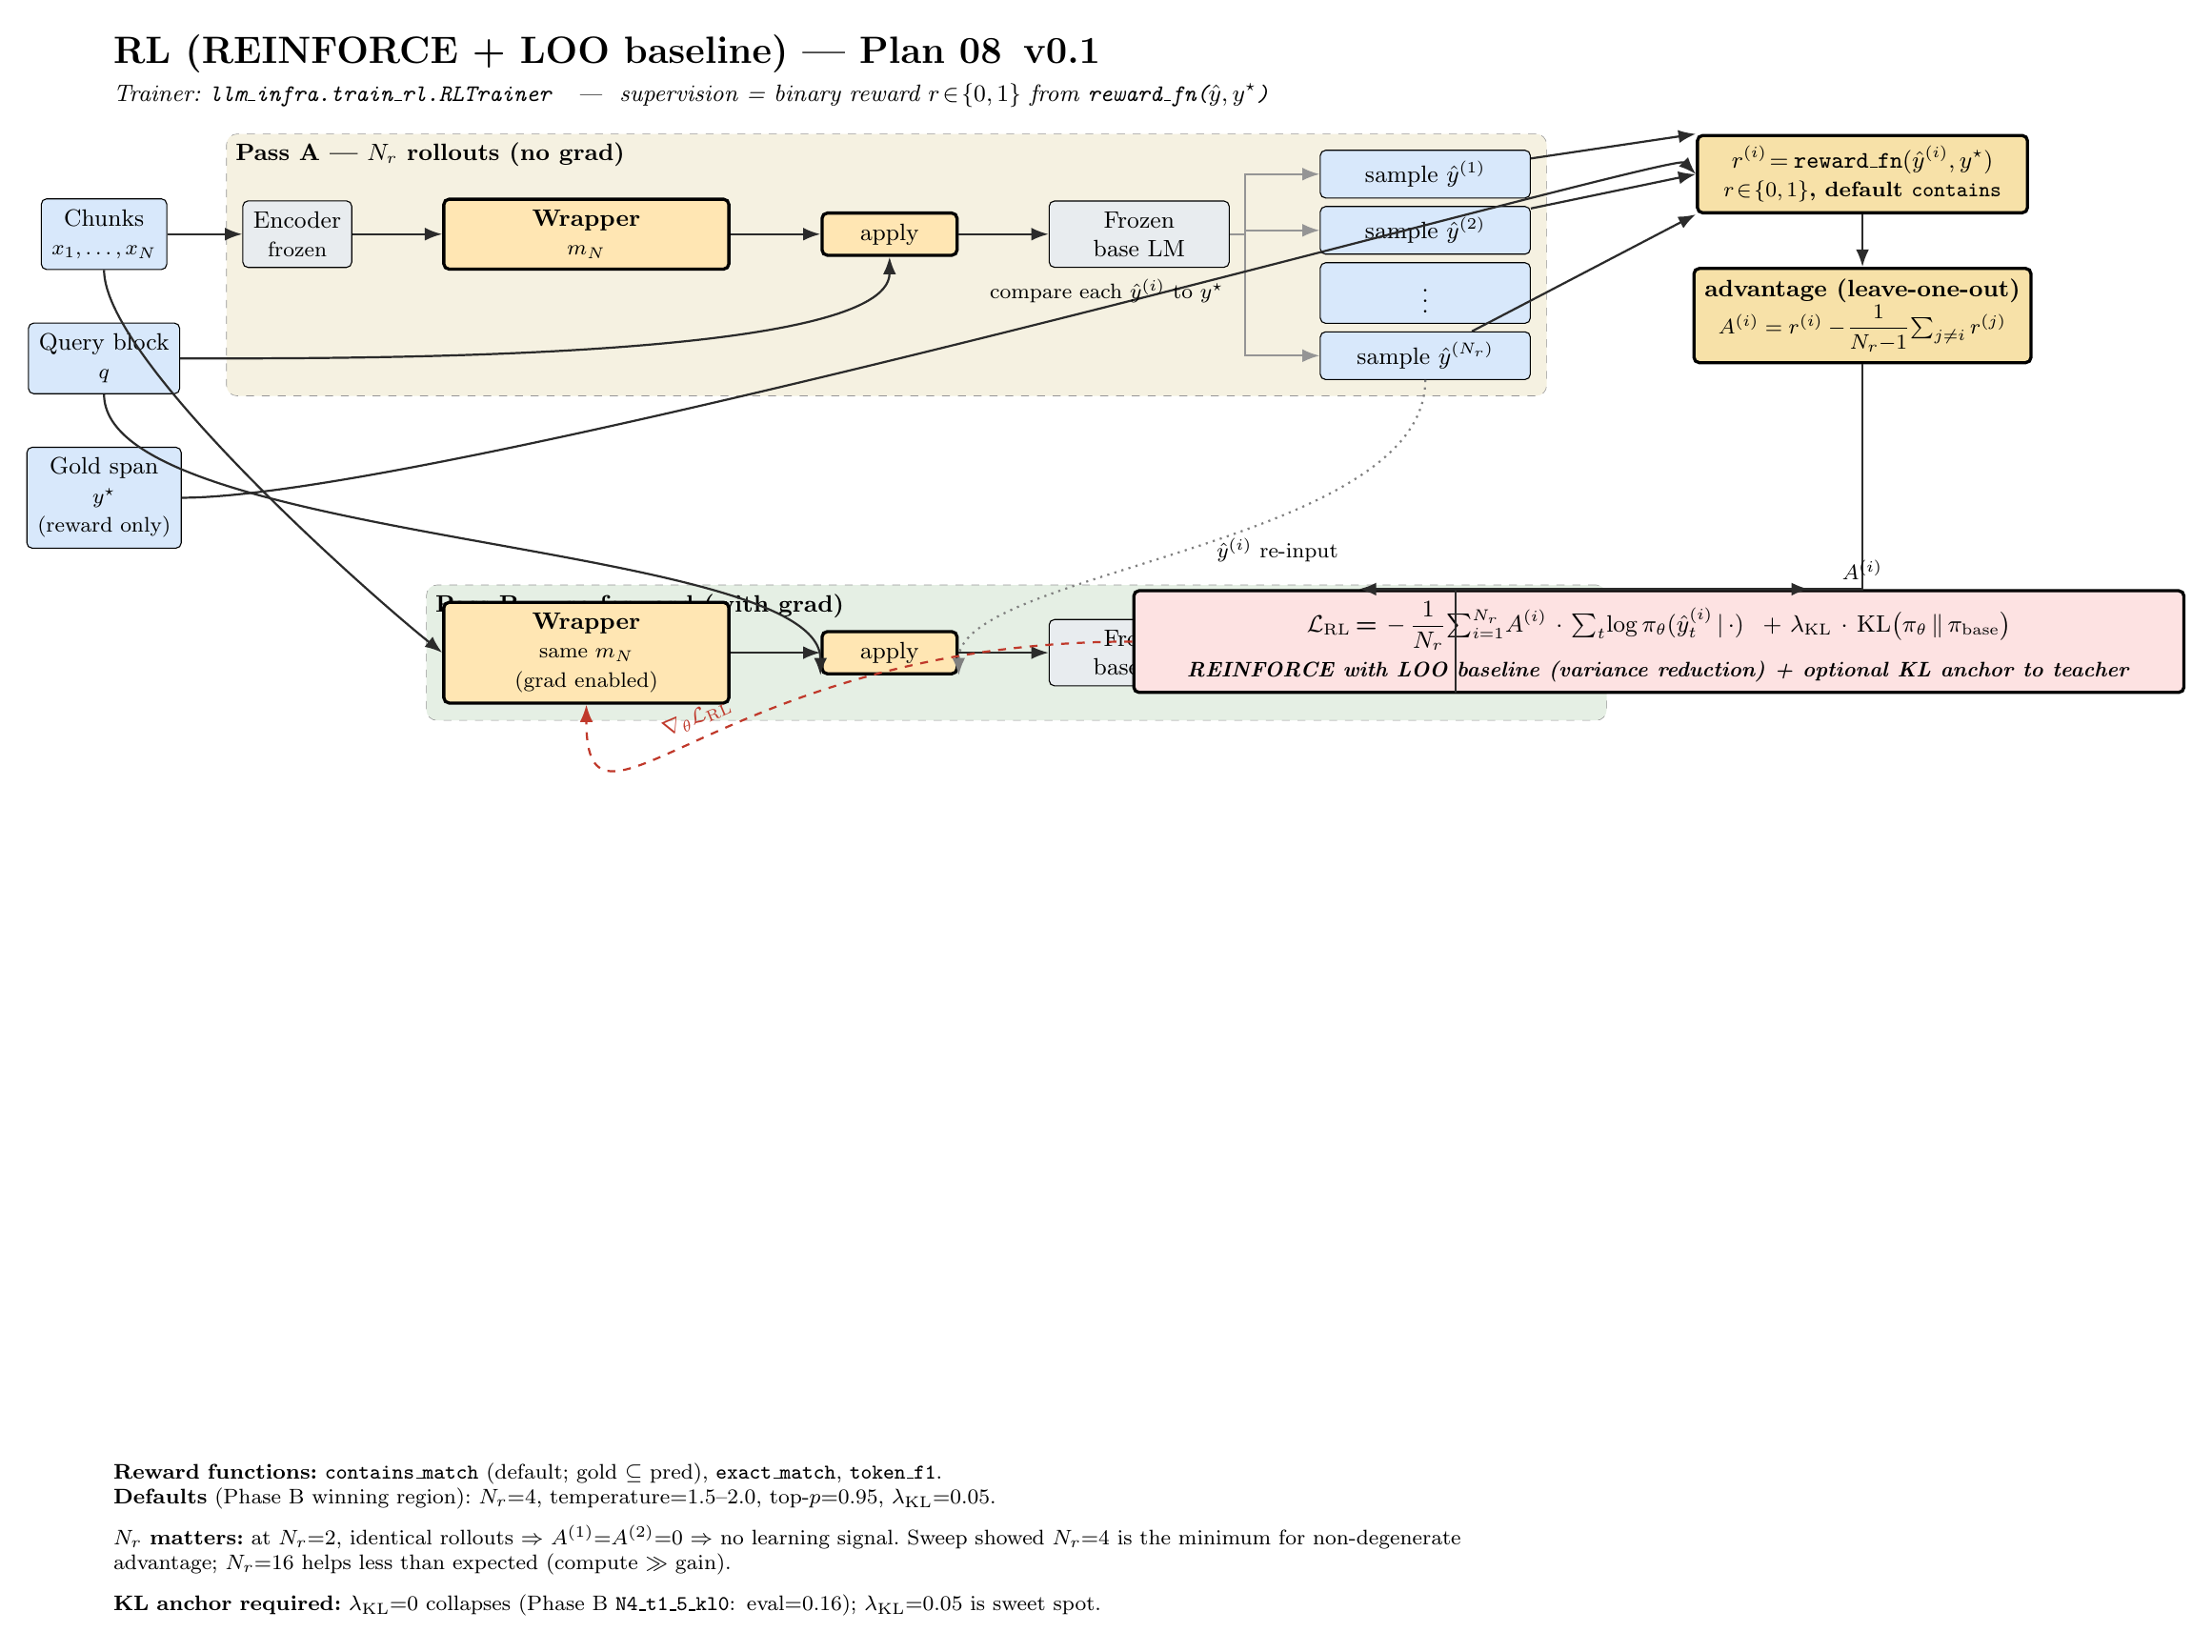
\begin{tikzpicture}[node distance=7mm and 12mm]

%% --- title -------------------------------------------------------------
\node[font=\Large\bfseries, anchor=west] (title) at (0,9.4)
  {RL (REINFORCE + LOO baseline) — Plan 08\ \,v0.1};
\node[font=\small\itshape, anchor=west] at (0,8.85)
  {Trainer:\ \texttt{llm\_infra.train\_rl.RLTrainer}\ \ \ |\ \
   supervision = binary reward $r\!\in\!\{0,1\}$ from \texttt{reward\_fn(}$\hat y, y^\star$\texttt{)}};

%% =====================================================================
%% Input
%% =====================================================================
\node[data] (chunks) at (0,7.0) {Chunks\\\footnotesize $x_1, \dots, x_N$};
\node[data, below=of chunks] (query) {Query block\\\footnotesize $q$};
\node[data, below=of query]  (gold) {Gold span\\\footnotesize $y^\star$\\\footnotesize (reward only)};

%% =====================================================================
%% Pass A — build memory + N rollouts (no grad)
%% =====================================================================
\node[frozen, right=10mm of chunks] (enc) {Encoder\\\footnotesize frozen};
\node[trained, right=of enc, minimum width=38mm] (wrap)
  {\textbf{Wrapper}\\\footnotesize $m_N$};
\node[trained, right=of wrap, minimum width=18mm] (apply) {apply};
\node[frozen, right=of apply, minimum width=24mm] (base)
  {Frozen\\base LM};

% N rollouts as a stack
\node[data, right=of base, yshift=8mm, minimum width=28mm]   (y1) {sample $\hat y^{(1)}$};
\node[data, below=1mm of y1,            minimum width=28mm] (y2) {sample $\hat y^{(2)}$};
\node[data, below=1mm of y2,            minimum width=28mm] (ydots) {\vdots};
\node[data, below=1mm of ydots,         minimum width=28mm] (yN) {sample $\hat y^{(N_r)}$};

\draw[flow] (chunks) -- (enc);
\draw[flow] (enc) -- (wrap);
\draw[flow] (wrap) -- (apply);
\draw[flow] (query.east) .. controls +(20mm,0) and +(0,-14mm) .. (apply.south);
\draw[flow] (apply) -- (base);
\draw[flow, draw=arrowclr!50] (base.east) -- ++(2mm,0) |- (y1.west);
\draw[flow, draw=arrowclr!50] (base.east) -- ++(2mm,0) |- (y2.west);
\draw[flow, draw=arrowclr!50] (base.east) -- ++(2mm,0) |- (yN.west);

\begin{pgfonlayer}{background}
  \node[passA, fit=(enc)(wrap)(apply)(base)(y1)(yN),
        label={[font=\small\bfseries, anchor=north west]north west:Pass A — $N_r$ rollouts (no grad)}] {};
\end{pgfonlayer}

%% =====================================================================
%% Reward + LOO baseline
%% =====================================================================
\node[reward, right=22mm of y1, minimum width=44mm] (rewards)
  {$r^{(i)} \!=\!$ \texttt{reward\_fn}$(\hat y^{(i)}, y^\star)$\\
   \footnotesize $r\!\in\!\{0,1\}$,\ default \texttt{contains}};
\node[reward, below=of rewards, minimum width=44mm] (advs)
  {advantage (leave-one-out)\\
   \footnotesize $A^{(i)} = r^{(i)} - \!\dfrac{1}{N_r{-}1}\!\sum_{j\neq i} r^{(j)}$};

\draw[flow] (gold.east) .. controls +(36mm,0) and +(-3mm,3mm) ..
   node[above,font=\footnotesize,xshift=10mm,yshift=2mm]{compare each $\hat y^{(i)}$ to $y^\star$}
   (rewards.west);
\draw[flow] (y1) -- (rewards.north west);
\draw[flow] (y2) -- (rewards.west);
\draw[flow] (yN) -- (rewards.south west);
\draw[flow] (rewards) -- (advs);

%% =====================================================================
%% Pass B — re-forward with grad → log-probs of rollouts
%% =====================================================================
\node[trained, below=44mm of wrap, minimum width=38mm] (wrap2)
  {\textbf{Wrapper}\\\footnotesize same $m_N$\\\footnotesize (grad enabled)};
\node[trained, right=of wrap2, minimum width=18mm] (apply2) {apply};
\node[frozen, right=of apply2, minimum width=24mm] (base2) {Frozen\\base LM};
\node[data, right=of base2, minimum width=36mm] (logp)
  {$\log\pi_\theta(\hat y^{(i)}_t\,|\,\cdot)$\\\footnotesize one re-fwd per rollout};

\draw[flow] (chunks.south) .. controls +(0,-12mm) and +(-10mm,8mm) .. (wrap2.west);
\draw[flow] (wrap2) -- (apply2);
\draw[flow] (query.south) .. controls +(0,-20mm) and +(0,18mm) .. (apply2.south west);
\draw[noflow] (yN.south) .. controls +(0,-22mm) and +(0,14mm) ..
   node[midway,right,font=\footnotesize,xshift=2mm]{$\hat y^{(i)}$ re-input} (apply2.south east);
\draw[flow] (apply2) -- (base2);
\draw[flow] (base2) -- (logp);

\begin{pgfonlayer}{background}
  \node[passB, fit=(wrap2)(apply2)(base2)(logp),
        label={[font=\small\bfseries, anchor=north west]north west:Pass B — re-forward (with grad)}] {};
\end{pgfonlayer}

%% =====================================================================
%% Loss
%% =====================================================================
\node[loss, below=14mm of $(advs)!0.5!(logp)$,
      minimum width=140mm, text width=136mm] (loss)
  {\textbf{$\mathcal{L}_{\mathrm{RL}}$\,=}\
   $-\,\dfrac{1}{N_r}\!\sum_{i=1}^{N_r}\!A^{(i)}\!\cdot\!\sum_{t}\!\log\pi_\theta(\hat y^{(i)}_t\,|\,\cdot)$
   \,\,$+\,\,\lambda_{\mathrm{KL}}\!\cdot\!\mathrm{KL}\bigl(\pi_\theta\,\|\,\pi_{\mathrm{base}}\bigr)$\\[1mm]
   \footnotesize\textit{REINFORCE with LOO baseline (variance reduction) + optional KL anchor to teacher}};

\draw[flow] (advs.south)  |- ($(loss.north)+(-40mm,0)$)
   node[midway,above,font=\footnotesize,sloped]{$A^{(i)}$};
\draw[flow] (logp.south)  |- ($(loss.north)+(20mm,0)$);

%% =====================================================================
%% Gradient
%% =====================================================================
\draw[grad] (loss.west) .. controls +(-55mm,0) and +(0,-22mm) .. (wrap2.south)
  node[midway,above,font=\footnotesize\bfseries,text=gradclr,sloped]
  {$\nabla_\theta\mathcal{L}_{\mathrm{RL}}$};

%% =====================================================================
%% Notes
%% =====================================================================
\node[font=\footnotesize, anchor=west, text width=185mm] at (0,-10.4)
  {\textbf{Reward functions:}\ \texttt{contains\_match} (default; gold $\subseteq$ pred),
   \texttt{exact\_match}, \texttt{token\_f1}.\\
   \textbf{Defaults} (Phase B winning region):\ $N_r{=}4$,\ temperature${=}1.5$\textendash$2.0$,\
   top-$p{=}0.95$,\ $\lambda_{\mathrm{KL}}{=}0.05$.\medskip\\
   \textbf{$N_r$ matters:}\ at $N_r{=}2$, identical rollouts $\Rightarrow$ $A^{(1)}{=}A^{(2)}{=}0$
   $\Rightarrow$ no learning signal.\ Sweep showed $N_r{=}4$ is the minimum for non-degenerate
   advantage; $N_r{=}16$ helps less than expected (compute $\gg$ gain).\medskip\\
   \textbf{KL anchor required:}\ $\lambda_{\mathrm{KL}}{=}0$ collapses (Phase B
   \texttt{N4\_t1\_5\_kl0}: eval${=}0.16$);\ $\lambda_{\mathrm{KL}}{=}0.05$ is sweet spot.};

\end{tikzpicture}
\end{document}
